\documentclass[a4paper]{proc}

\usepackage[utf8]{inputenc}
\usepackage[T1]{fontenc}
\usepackage[english]{babel}
\usepackage{graphicx}
\usepackage{url}
\usepackage{mathtools}
\usepackage{indentfirst}
\counterwithin*{section}{part}


\author{Paul MABILEAU\\\texttt{paul.mabileau@telecom-sudparis.eu}
        \and Franck STAUFFER\\\texttt{franck.stauffer@telecom-sudparis.eu}}
\title{\textbf{Recursive Inter-Network Architecture's Security}}

\begin{document}
\maketitle
\tableofcontents
\newpage
\part{Introduction}

The Recursive Inter-Network Architecture (RINA) is a network architecture born
in John Day's \texttt{Patterns in Network Architecture: A Return to
Fundamentals} in 2008.  It emerges from the fact that TCP/IP was designed a
while ago without security in mind and that the huge amount of RFCs\cite{rfc}
published since 1969 by the IETF to add security in it created
complexity.\cite{assessing-security} Moreover the book states that the current
internet architecture is not an actual `inter-net' but more a juxtaposition of
different networks on a same bigger network.

To remedy, it proposes to go back to fundamentals and states that networking is
only Inter Process Communication (IPC) and thus John Day proposed the Recursive
InterNetwork Architecture (RINA) as an alternative.  RINA promises to reduce
complexity by reducing the number of protocols, separating mechanisms and
policies, using connection-less communications and reworking the whole way
things work.  This architecture claims to be more secure by design than the
TCP/IP architecture.

The architecture is also developped by the Pouzin Society\cite{psoc} that kind
of replace the IETF by publishing specifications.  Some simulations and studies
have been lead in Europe with IRATI\cite{web:irati} and PRISTINE\cite{pristine}
for example.  You can also find a framework to test RINA on OMNeT++ named
RINASim at \url{https://rinasim.omnetpp.org/}.

First we will provide a presentation of the RINA architecture, then we will
discuss its security compared to the TCP/IP architecture.

\newpage
\part{Comparing RINA and TCP/IP}
\section{Architecture}

RINA uses a single recursive layer named a Distributed IPC Facility (DIF). It
can be stacked as much as needed by the network architecture instead of being a
static model like in TCP/IP\@.  Inside the DIFs there are IPC Processes (IPCPs)
that communication using a Common Distributed Application Protocol (CDAP) that
only allows six basic operations to be used on a remote object
\cite{Trouva2011ISTI}:

\begin{itemize}
    \item Allocate
    \item Send
    \item Receive
    \item Deallocate
\end{itemize}

Those IPCPs deal with tasks which can be divided in three parts (figure
\ref{fig:arch}).  The parts are ordered from the less complex and more frequent
to the more complex and less frequent ones:

\begin{itemize}
    \item Data Transfer: it deals with SDU delimiting (fragmentation,
        concatenation, separationm, reassembly), SDU Protection (integrity/error
        detection), Relaying and Multiplexing Task and actual Data Transfer
        \cite{irati}.
    \item Data Transfer Control: it deals with Transmission Control,
        Retransmission Control and Flow Control.
    \item Layer Management: it deals with Authentication, Enrollment, Namespace
        Management, Flow Allocation, Forwarding Table Generator, Resource
        Allocation, Security Management and CDAP Parsing and Generation.
\end{itemize}

The $N-DIF$ only knows $(N + 1)-DIF$ and $(N - 1)-DIF$\@.  The $(N + 1)-DIF$ is
saw as an Application Process (AP) because all IPCPs are actually APs.  There is
one exception to this rule, there is a special DIF that is called a Distributed
Application Facility (DAF) that has no $(N + 1)-DIF$\@.  This DIF is composed of
one or more Distributed Application Processes (DAPs) in place of IPCPs.  This
DIF can be considered as the Application layer from the TCP/IP model.  IPCPs
only communicates with other IPCPs in the same DIF like in the TCP/IP model with
layers.  IPCs communicate in the form of Protocol Data Units (PDUs) that contain
a header or a trailer (named Protocol Control Information (PCI)), and a
payload.\cite{PINS} The DIFs choose to use a connection-oriented or a
connection-less communication depending on the needs of the IPCP\@.

\begin{figure}
    \centering
    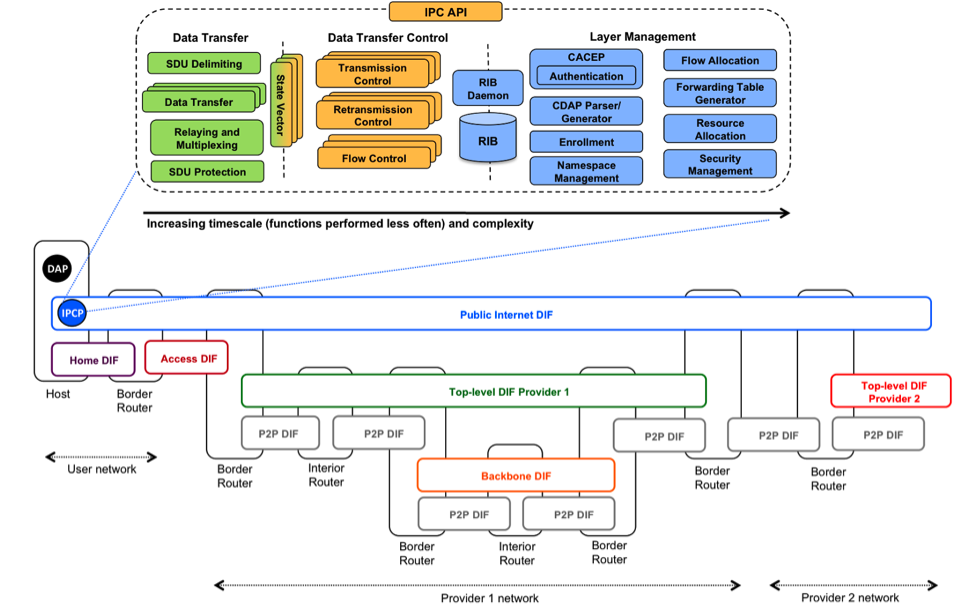
\includegraphics[width=\columnwidth]{arch.png}
    \caption{RINA's architecture}
    \label{fig:arch}
\end{figure}

\section{Delta-t synchronization}

According to RINASim's webpage: `There is no need for explicit state
synchronization (hard-state) and tools like SYNs and FINs are unnecessary'.
Instead they use the Delta-t transport protocol\cite{65288}.  It is a time-based
synchronization techniques that only needs 3 timers:

\begin{itemize}
    \item Maximum Packet Lifetime
    \item Maximum time to attempt retransmission
    \item Maximum time before Acknowledgement
\end{itemize}

In this protocol, every connections exists at every point in time.  When there
is no traffic the synchronization state is maintained during 2 or 3 Maximum
Packet Lifetimes.\cite{rinasim}

\section{Naming and adressing}

To replace the IP, each IPCP has an variable length address that is visible only
in the DIF in which it is.  The length of the address is variable but all IPCPs
in the DIF have the same address length so it is a parameter of the DIF itself.
When two applications wants to communicate, their underlying DIF knows on which
IPCP each of them is connected.  So the the apllication that is going to open
communication does an allocate request to its Point of Attachement (PoA, the
IPCP to which it is connected).  This PoA calls its Flow Allocator to verify the
request and to verify that enough resources are available.  If it is accepted,
it seeks for a mapped entry in the local directory if there is an IPCP that is
connected to the other application.  If it finds one, it sends a request to
create a flow with a CDAP exchange protocol.  When the PoA of the target
application receives the request, it forwards it to the application.  If the
source application has access rights to the target application, the former asks
to its PoA to allocate resources for the flow.  Then the PoA sends a CDAP
response to the other one.  Now the applications can send and receive SDU using
the the IPC API\@.  At the end of the communication they release the allocated
resources using this same API\@.\cite{Trouva2011ISTI}


\part{Security provided by RINA's conception}

In this part, we will study how RINA's design can help in preventing various
types of attacks through simple and elementary considerations. We will also see
how the current model for network communications has trouble protecting itself
from such attacks. This is often the approach used in articles assessing RINA's
global and general security by comparing current possibilities with the RINA
model and by trying to re-create these attacks, sometimes theoretically.

\section{Authentication}

In RINA, authentication is mandatory. This is one of the major, if not the most
important security feature of the architecture, as previous security analysis
often consider attacks plausible only after a successful authentication
\cite{assessing-security, wiki, PINS}.

Authentication occurs before a process may communicate on a DIF, either by
creating a new one, or by joining an existing one, and is verified by the
destination application process. When creating a brand new DIF, the initial IPC
process simply has to exist in order to let others join the newly created DIF.
When joining an already existing DIF, the joining process asks permission to the
destination process it wants to communicate with. It achieves this using a
subsequent DIF that both processes have in common and are authenticated in.  The
destination process is the one that determines whether the joining one has
sufficient rights through any sort of authentication, described in the DIF's
policy. It may be as strong or weak as desired by the DIF and for the wanted
communication. Then, the destination process gives the joining one a new node
address so it may communicate on the newly joined DIF with.

This design feature is quite useful for hardening security considerations in
network communications, as being authenticated \textit{every time} means that
the destination application decides who to talk with and how strict this
decision is using policies, \textit{every time}. It thus builds greater trust
between applications through native access control.

\section{Strict encapsulation}

Encapsulation is a very common paradigm for network communications, as it helps
in keeping functionally different parts of the global system separate in
conception as well as in usage. However, the historical TCP/IP model chose to
apply this by function rather than by scope. This means that separation of
concerns is relatively poorly achieved because a certain layer needs to know a
certain amount of information about its subsequent layer(s) in order to properly
work and deliver the expected service. For example, when establishing an HTTP
connection, the client has to:
\begin{enumerate}
    \item Resolve the IP address through the \textit{Domain Name System} (DNS).
        One could argue that this constitutes a two-level layer leakage, as it
        crosses TCP and IP.
    \item Use the resulting IP address in the transport layer (TCP) in order to
        establish a connection.
    \item Suppose the correct destination port using well-known ports.
\end{enumerate}
This renders the communication not ideal.

On the contrary, RINA deals with layers in a stricter way: a process may only
use the functions of a DIF below it is connected to and serve the application
that is above it. It is not supposed to guess or determine information about
inferior or superior DIFs. This is the recursive property of RINA. Although it
may seem simple, it is a fundamental rewind: at any level in the communications
stack a DIF can decide to encrypt or hash its data units if it does not trust
its inferior DIF in order to achieve confidentiality or integrity. One can thus
easily imagine the amount of protection reinforcements that can be achieved with
this, which could be loosely compared to \textit{The Onion Router} (TOR) project
that offers many public and free network relays so users may connect to a remote
web site only through a circuit of these machines with additional encryption
between each of them. This project exists mainly for privacy concerns, but it
still illustrates the possibilities at hand.

\section{Soft-state communication}

All communication protocols meant to be used in RINA are designed to have soft
states instead of hard states. That is to say, connections are not established
with handshakes and terminated with explicit control messages or other types of
marital negociations, contrary to strongly connected protocols like TCP. In
RINA, data transfers use the Delta-T protocol \cite{delta-t}, which is based on
a couple of timers to check the state of the connection. Given a \textit{Maximum
Packet Lifetime} (MPL) as defined by the IPC process in the security policy, $2
\times MPL$ after a packet has been received by the recipient or $3 \times MPL$
after the sender last emitted a packet and received its corresponding
\textit{ACK}, the connection is closed without any form of exchange to do so.

In the traditional model of the Internet, there are two mainstream protocols
used for the transport layer: TCP and UDP. As we already illustrated, TCP is
mainly a hard-state connected protocol. UDP is a connectionless protocol, which
makes it quite simple but as there is no traffic control, it is best suited for
real-time transfers that can afford loosing a limited quantity of information
along the way. Therefore, Delta-T in RINA offers an in-between: messages are
assured to arrive to their destination through positive acknowledgment of every
message, but connections are managed on both ends using simple timer-based
mechanisms.

These considerations effectively protect communications in general. Indeed, the
requirement for an explicitly transfered connection management exposes a major
attack vector: port scanning, identity impersonation, data injection, denial of
service, ... These attacks are not necessarily easy, but still are elementary,
especially the first and last ones. Strictly timer-based handling thus avoids
risking some sorts of connection manipulation and offers a cleaner way of
communicating. Note that TCP was originally designed to only use the explicit
control messages in order to handle connections and manage data flows, but many
network-related hazards revealed flaws in this type of control, making it
ineffective. TCP's designers then had to include timer-based and other
mechanisms in order to circumvent these problems \cite{delta-t}. So not only
Delta-T makes communicating simpler and cleaner in basic network terms only, it
also solves quite a few issues related to network and applications security.


\nocite{*}
\newpage
\bibliographystyle{unsrt}
\bibliography{report}
\end{document}
